\documentclass{beamer}

%% Juego de caracteres usado en el archivo fuente: UTF-8
\usepackage{ucs}
\usepackage[utf8x]{inputenc}
\uselanguage{spanish}
%Para la identación del español
\usepackage[spanish]{babel}
\usepackage{animate}

% There are many different themes available for Beamer. A comprehensive
% list with examples is given here:
% http://deic.uab.es/~iblanes/beamer_gallery/index_by_theme.html
% You can uncomment the themes below if you would like to use a different
% one:
%\usetheme{AnnArbor}
%\usetheme{Antibes}
%\usetheme{Bergen}
%\usetheme{Berkeley}
%\usetheme{Berlin}
%\usetheme{Boadilla}
%\usetheme{boxes}
%\usetheme{CambridgeUS}
%\usetheme{Copenhagen}
%\usetheme{Darmstadt}
%\usetheme{default}
%\usetheme{Frankfurt}
%\usetheme{Goettingen}
%\usetheme{Hannover}
%\usetheme{Ilmenau}
%\usetheme{JuanLesPins}
%\usetheme{Luebeck}
\usetheme{Madrid}
%\usetheme{Malmoe}
%\usetheme{Marburg}
%\usetheme{Montpellier}
%\usetheme{PaloAlto}
%\usetheme{Pittsburgh}
%\usetheme{Rochester}
%\usetheme{Singapore}
%\usetheme{Szeged}
%\usetheme{Warsaw}

%Para la identación del español
\usepackage[spanish]{babel}

\title{¿Estamos seguros en una red WiFi?}

% A subtitle is optional and this may be deleted
%\subtitle{Optional Subtitle}

\author{Jesús Rodríguez Heras \\ Juan Pedro Rodríguez Gracia}
% - Give the names in the same order as the appear in the paper.
% - Use the \inst{?} command only if the authors have different
%   affiliation.

%\institute[Escuela Superior de Ingeniería] % (optional, but mostly needed)
%{
%  \inst{1}%
%  Department of Computer Science\\
%  University of Somewhere
%  \and
%  \inst{2}%
%  Department of Theoretical Philosophy\\
%  University of Elsewhere}
% - Use the \inst command only if there are several affiliations.
% - Keep it simple, no one is interested in your street address.

\date{8 de mayo de 2018}
% - Either use conference name or its abbreviation.
% - Not really informative to the audience, more for people (including
%   yourself) who are reading the slides online

%\subject{Theoretical Computer Science}
% This is only inserted into the PDF information catalog. Can be left
% out. 

% If you have a file called "university-logo-filename.xxx", where xxx
% is a graphic format that can be processed by latex or pdflatex,
% resp., then you can add a logo as follows:

% pgfdeclareimage[height=0.5cm]{university-logo}{university-logo-filename}
% \logo{\pgfuseimage{university-logo}}

% Delete this, if you do not want the table of contents to pop up at
% the beginning of each subsection:
%\AtBeginSubsection[]
%{
%  \begin{frame}<beamer>{Índice}
%    \tableofcontents[currentsection,currentsubsection]
%  \end{frame}
%}

% Let's get started
\begin{document}

\begin{frame}
  \titlepage
%  \begin{center}
%  
\includegraphics[scale=0.2]{Portada.png}	
%  \end{center}
  
\end{frame}

\begin{frame}{Índice}
  \tableofcontents
  % You might wish to add the option [pausesections]
\end{frame}

% Section and subsections will appear in the presentation overview
% and table of contents.


%\section{Eavesdropping en red abierta}
%\begin{frame}{Eavesdropping en red abierta}
%	\begin{block}{Definición}
%		Es un ataque donde el hacker puede leer los datos recibidos de una víctima a voluntad. Dicho atacante se coloca entre el emisor original del mensaje y el receptor original del mismo sin que ninguno de ellos sepa de la existencia del atacante. Debido a esto, ninguna de las partes sabe que el mensaje enviado/recibido ha sido violado por el atacante.
%	\end{block}
%	\begin{center}
%		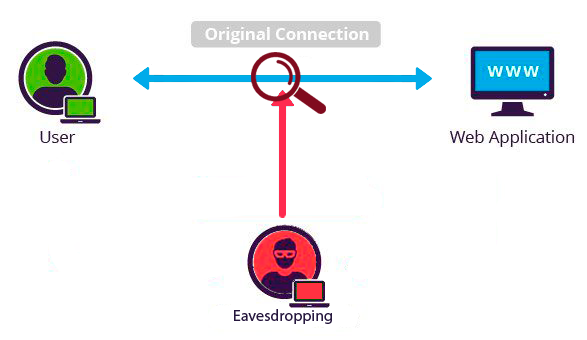
\includegraphics[scale=0.35]{EavesDropping.png}
%	\end{center}
%\end{frame}
%
%\begin{frame}{Ejemplo con Ettercap en red abierta}
%\begin{block}{¿Qué es Ettercap?}
%	Es un sniffer para redes LAN que permite la lectura, inyección y modificación de datos en una conexión entre el emisor y el receptor de un mensaje.
%\end{block}
%\begin{block}{¿Cómo funciona?}
%	Para el ejemplo en el que nos vamos a centrar, simplemente usaremos un ataque ``Eavesdropping'' para la lectura de las credenciales de usuario en una página web con protocolo HTTP debido a que las páginas que usan HTTPS tienen un cifrado de credenciales y no podemos acceder a ellas.
%\end{block}
%\end{frame}
%
%
%
%\begin{frame}{Ejemplo con Ettercap en red abierta}
%\begin{columns}
%	\column{0.45\textwidth}
%	
%	\begin{block}{Paso 1}
%		\begin{center}
%			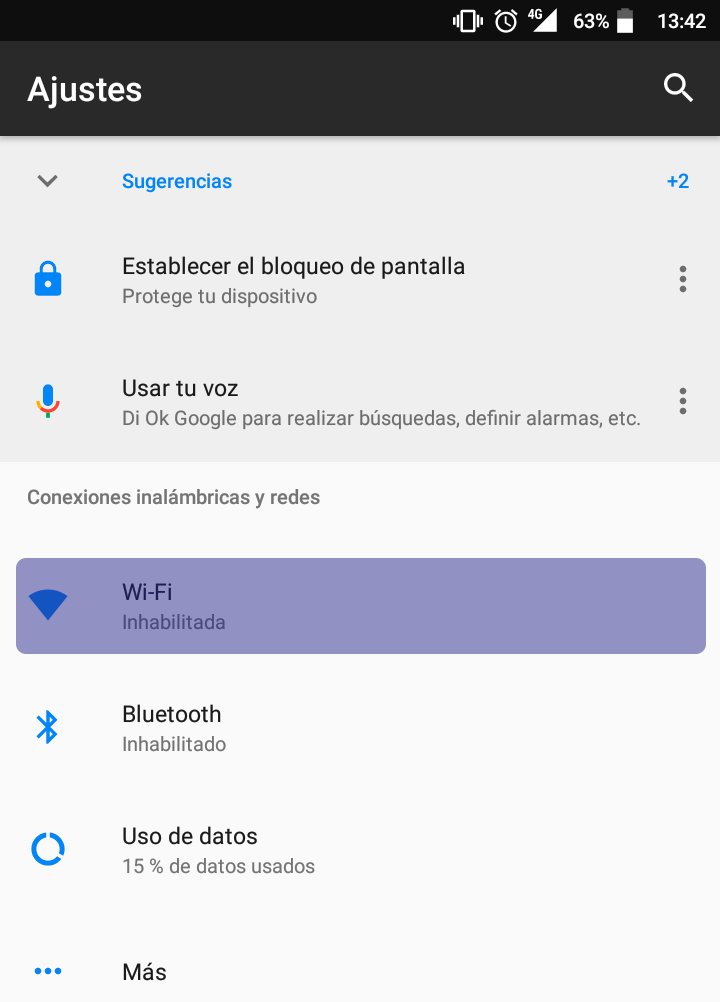
\includegraphics[scale=0.18]{1.png}
%		\end{center}
%	\end{block}
%\column{0.45\textwidth}
%\begin{block}{Paso 2}
%	\begin{center}
%		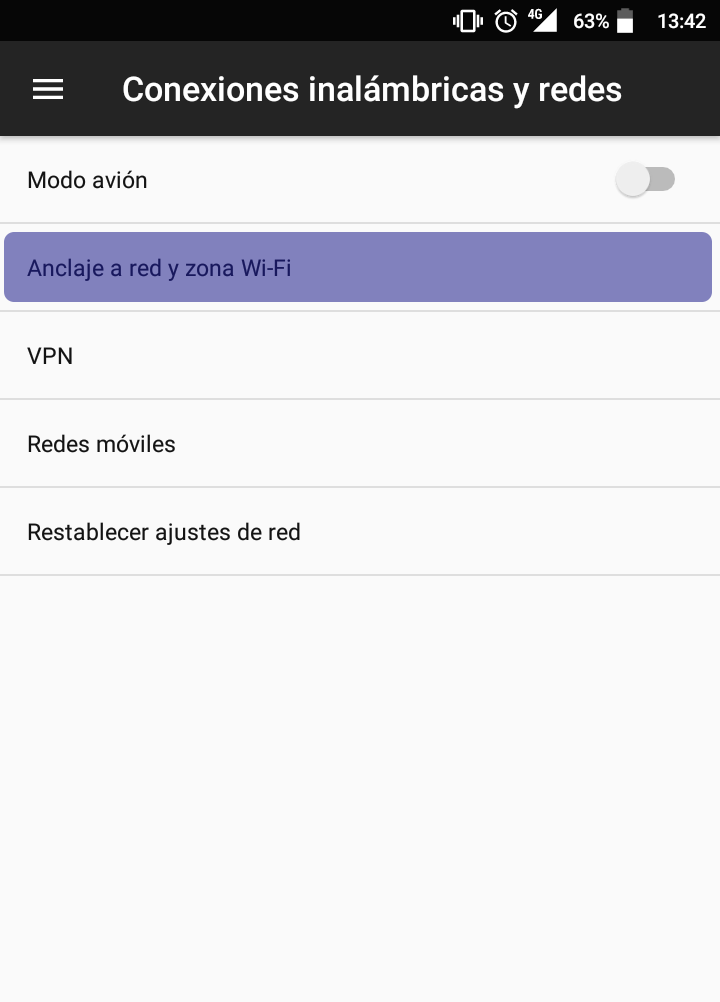
\includegraphics[scale=0.18]{2.png}
%	\end{center}
%\end{block}
%\end{columns}
%\end{frame}
%
%\begin{frame}{Ejemplo con Ettercap en red abierta}
%\begin{columns}
%\column{0.45\textwidth}
%\begin{block}{Paso 3}
%\begin{center}
%	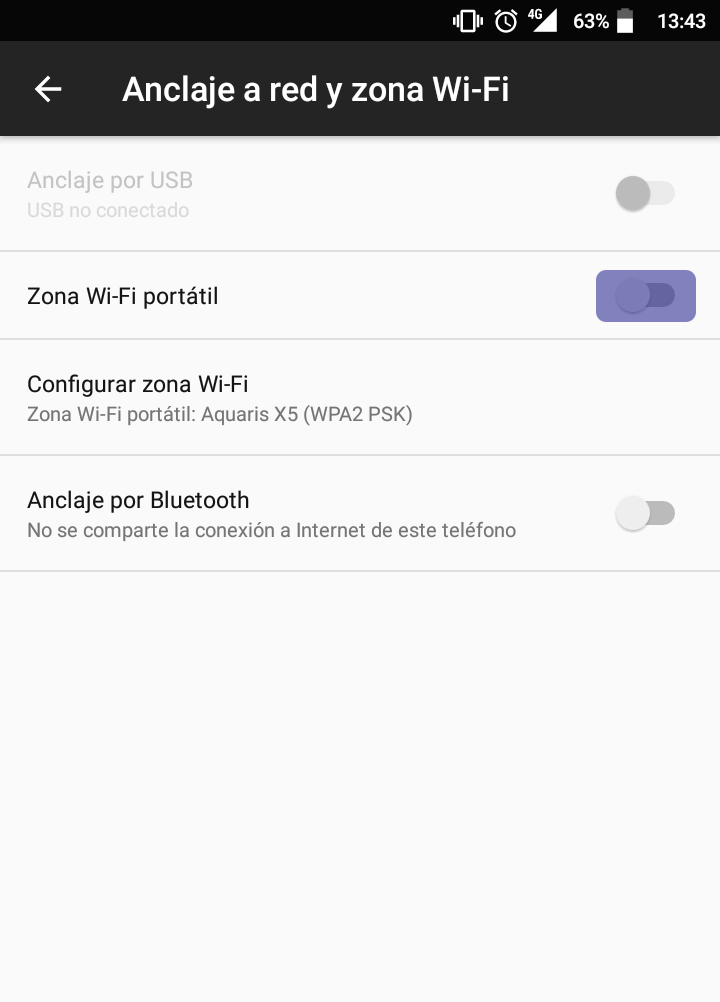
\includegraphics[scale=0.18]{3.png}
%\end{center}
%\end{block}
%\column{0.45\textwidth}
%\begin{block}{Paso 4}
%	\begin{center}
%		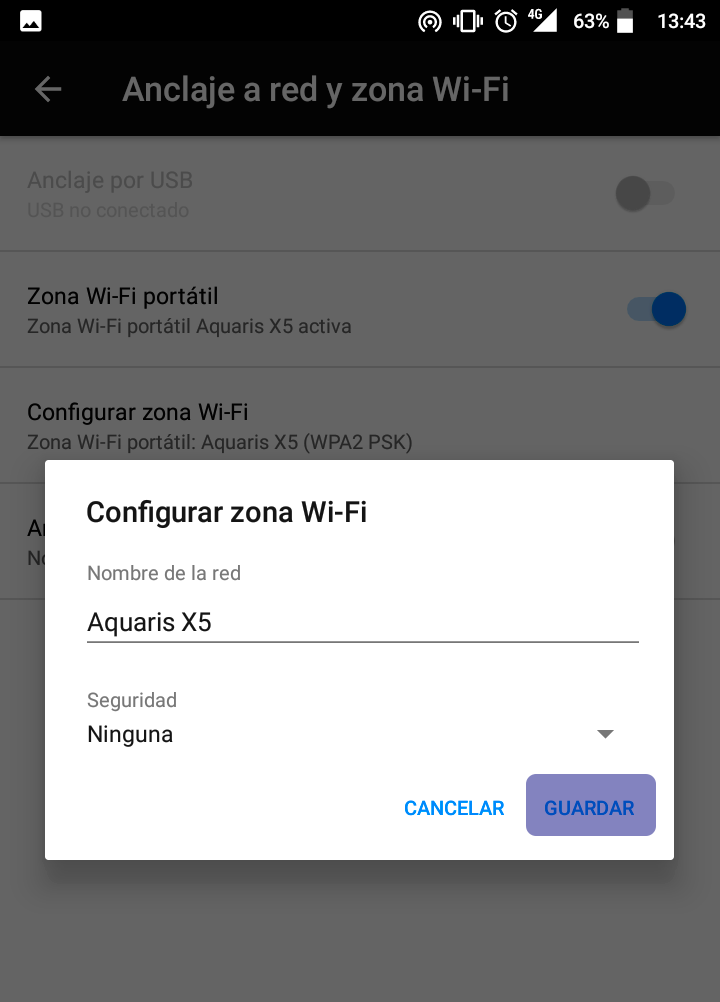
\includegraphics[scale=0.18]{4v1.png}
%	\end{center}
%	
%\end{block}
%
%\end{columns}
%\end{frame}
%
%\begin{frame}{Ejemplo con Ettercap en red abierta}
%\begin{columns}
%	\column{0.45\textwidth}
%	\begin{block}{Paso 3}
%		\begin{center}
%			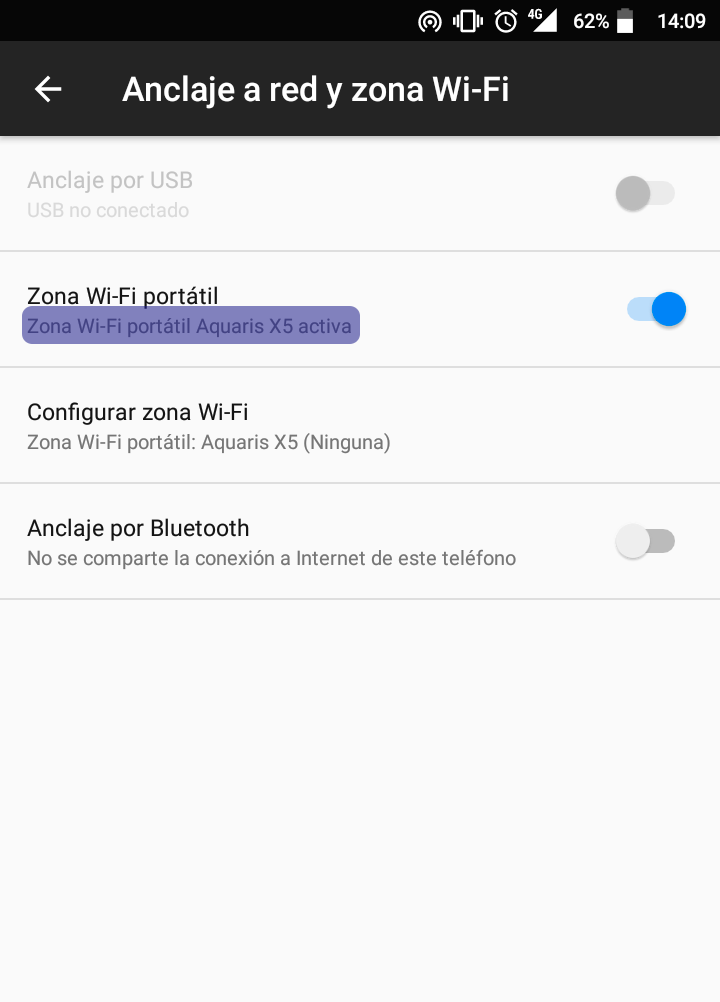
\includegraphics[scale=0.18]{5v1.png}
%		\end{center}
%	\end{block}
%\end{columns}
%\end{frame}
%
%\begin{frame}{Ejemplo con Ettercap en red abierta}
%\begin{block}{Escenario}
%	\begin{center}
%		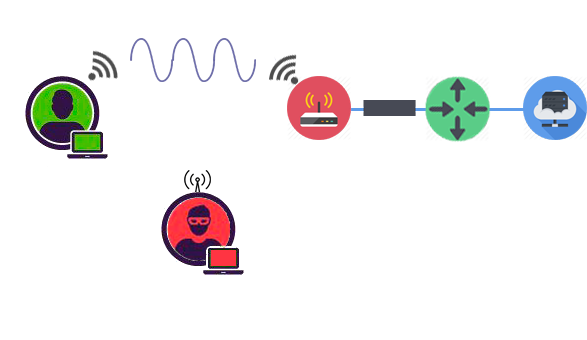
\includegraphics[scale=0.55]{RedSinCandados.png}
%	\end{center}
%\end{block}	
%\end{frame}
%
%\begin{frame}{¿Qué ha pasado?}
%	\begin{alertblock}{Explicación}
%		Hoy en día, muchas tarjetas de red poseen un filtro que impide el modo promiscuo y, por lo tanto, el eavesdropping.\\
%		Otro impedimento importante a la hora de realizarlo en windows es su firewall que puede impedir conexiones en redes abiertas.
%	\end{alertblock}
%\end{frame}



\section{WPA2-PSK}
\begin{frame}{WPA2-PSK}
\begin{block}{¿Qué es WPA2-PSK?}
	Es un protocolo de seguridad que cifra los mensajes en las redes inalámbricas (Wi-Fi) para permitir comunicaciones seguras.
\end{block}
\begin{center}
	
\includegraphics[scale=0.35]{wpa2.png}
\end{center}
\end{frame}

\section{Espionaje en red WPA2-PSK}
\begin{frame}{Espionaje en red WPA2-PSK}
Se nos presentan dos situaciones:
\begin{enumerate}
	\item Conocemos la passphrase (contraseña WiFi).
	\item No conocemos la passphrase (contraseña WiFi).
\end{enumerate}
\end{frame}

\subsection{Conocemos la passphrase}
\begin{frame}{Espionaje en red WPA2-PSK}
	Se nos presentan dos situaciones:
	\begin{enumerate}
		\item \textbf{{\large Conocemos la passphrase.}}
		\item No conocemos la passphrase.
	\end{enumerate}
\end{frame}

\begin{frame}{Espionaje en red WPA2-PSK conociendo la passphrase}
\begin{block}{ARP Poisoning}
	Es un ataque en el cual se busca engañar a un dispositivo modificando su tabla ARP.  En concreto en nuestro ataque buscamos engañar a la victima para poder recibir el tráfico.
\end{block}
\end{frame}

\begin{frame}{ARP Poisoning}
\begin{block}{Paso 1. ARP Replay para envenenar la tabla ARP de la víctima}
%		ARP Replay para envenenar la tabla ARP de la víctima.
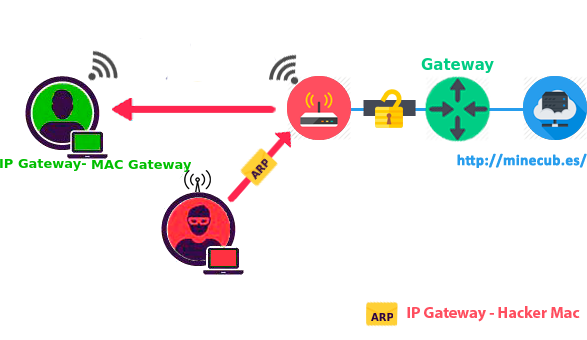
\includegraphics[scale=0.55]{ARPpoison1.png}
\end{block}
\end{frame}

\begin{frame}{ARP Poisoning}
\begin{block}{Paso 2. La víctima modifica su tabla ARP}
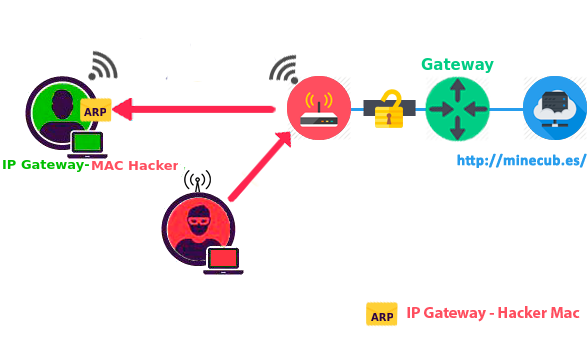
\includegraphics[scale=0.55]{ARPpoison2.png}
\end{block}
\end{frame}

\begin{frame}{ARP Poisoning}
\begin{block}{Paso 3. La víctima lanza una solicitud HTTP}
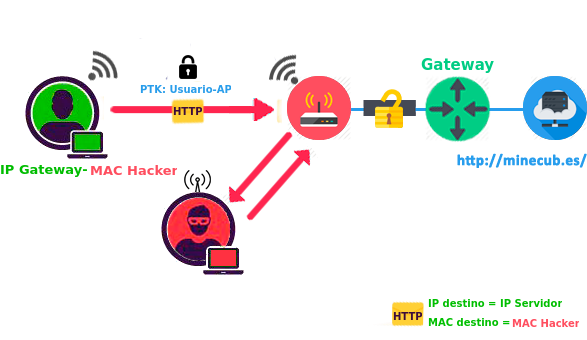
\includegraphics[scale=0.55]{ARPpoison3.png}
\end{block}
\end{frame}

\begin{frame}{ARP Poisoning}
\begin{block}{Paso 4. El AP redirecciona el paquete a la MAC del hacker}
	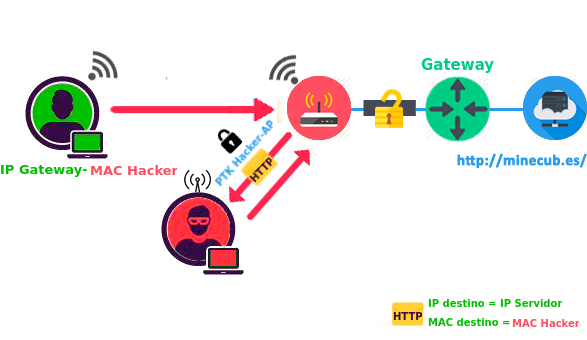
\includegraphics[scale=0.55]{ARPpoison3-2.png}
\end{block}
\end{frame}

\begin{frame}{ARP Poisoning}
\begin{block}{Paso 5. El hacker lee y envía el paquete al destinatario legítimo}
	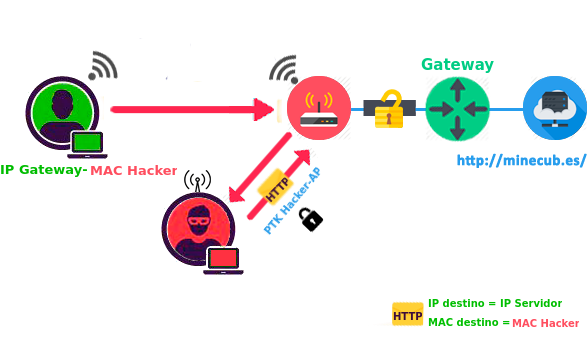
\includegraphics[scale=0.55]{ARPpoison3-3.png}
\end{block}
\end{frame}

\begin{frame}{Ejemplo con Ettercap en red segura}
\begin{columns}
	\column{0.45\textwidth}

\begin{block}{Paso 1}
	\begin{center}
		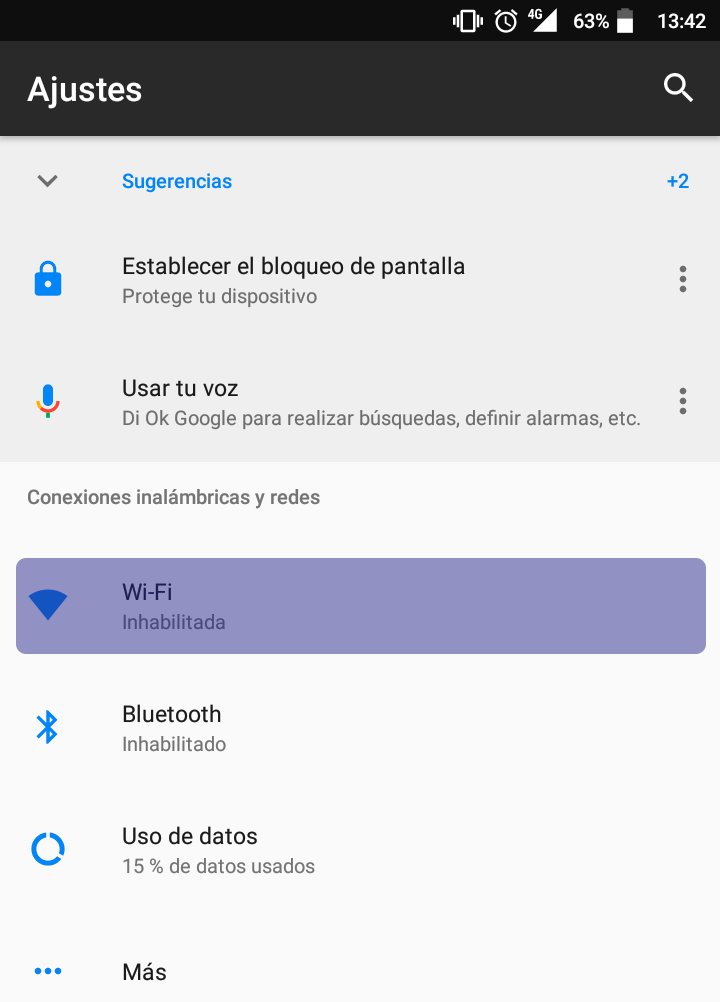
\includegraphics[scale=0.18]{1.png}
	\end{center}
\end{block}
\column{0.45\textwidth}
\begin{block}{Paso 2}
	\begin{center}
		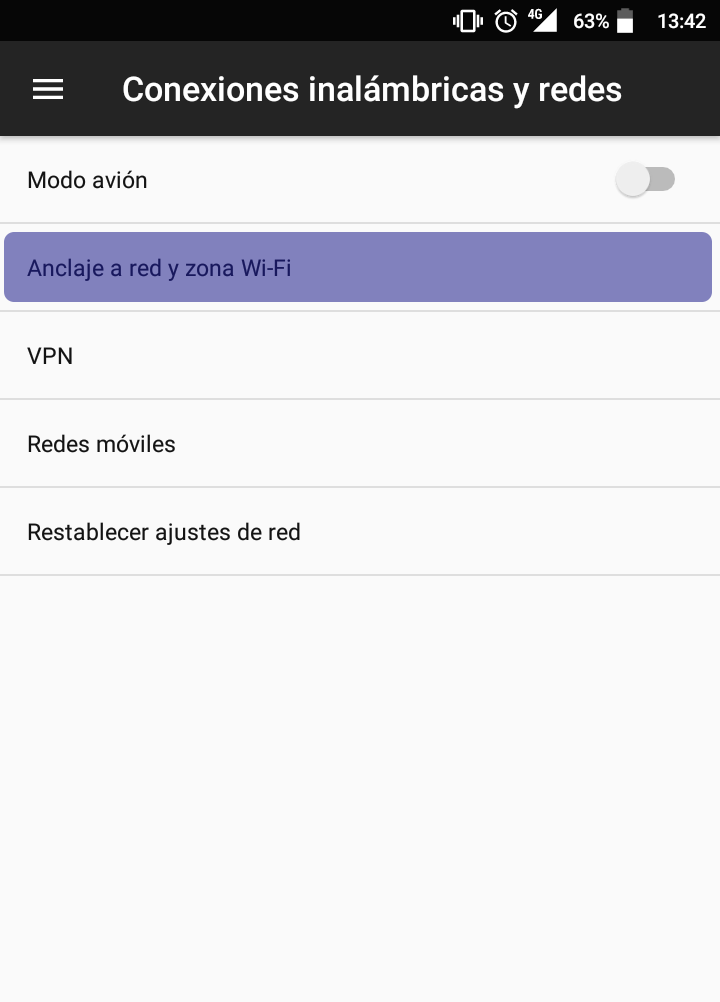
\includegraphics[scale=0.18]{2.png}
	\end{center}
\end{block}
\end{columns}
\end{frame}


\begin{frame}{Ejemplo con Ettercap en red segura}
\begin{columns}
	\column{0.45\textwidth}
\begin{block}{Paso 3}
	\begin{center}
		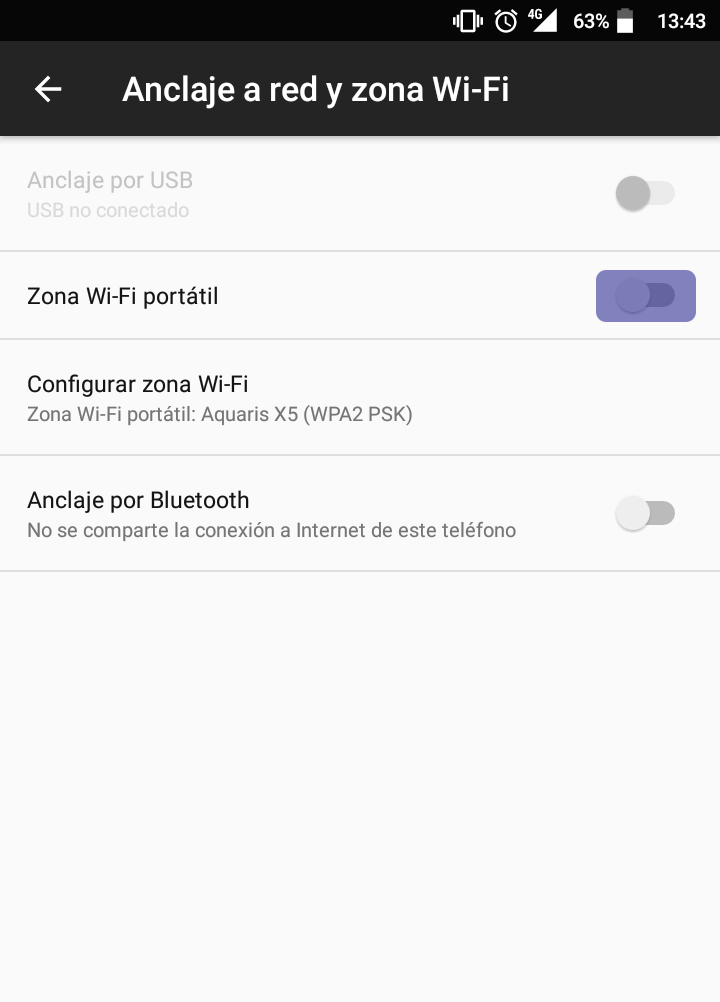
\includegraphics[scale=0.18]{3.png}
	\end{center}
\end{block}
\column{0.45\textwidth}
\begin{block}{Paso 4}
	\begin{center}
		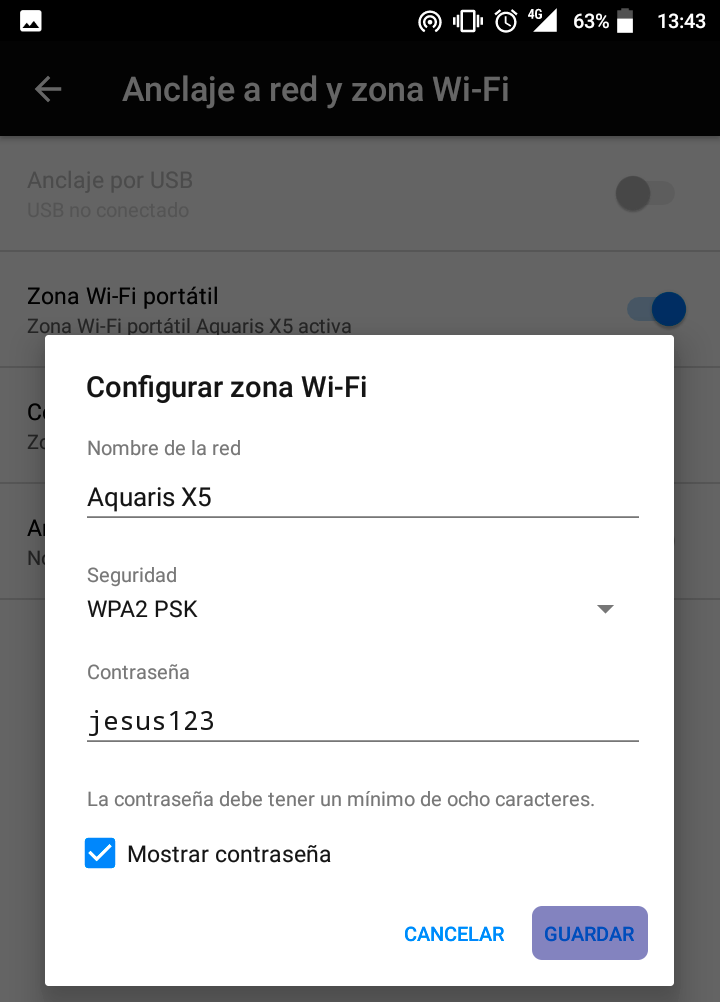
\includegraphics[scale=0.18]{5v2.png}
	\end{center}
	
\end{block}

\end{columns}
\end{frame}


\begin{frame}{Ejemplo con Ettercap en red segura}
\begin{columns}
	\column{0.45\textwidth}
	\begin{block}{Paso 5. Red segura}
		\begin{center}
			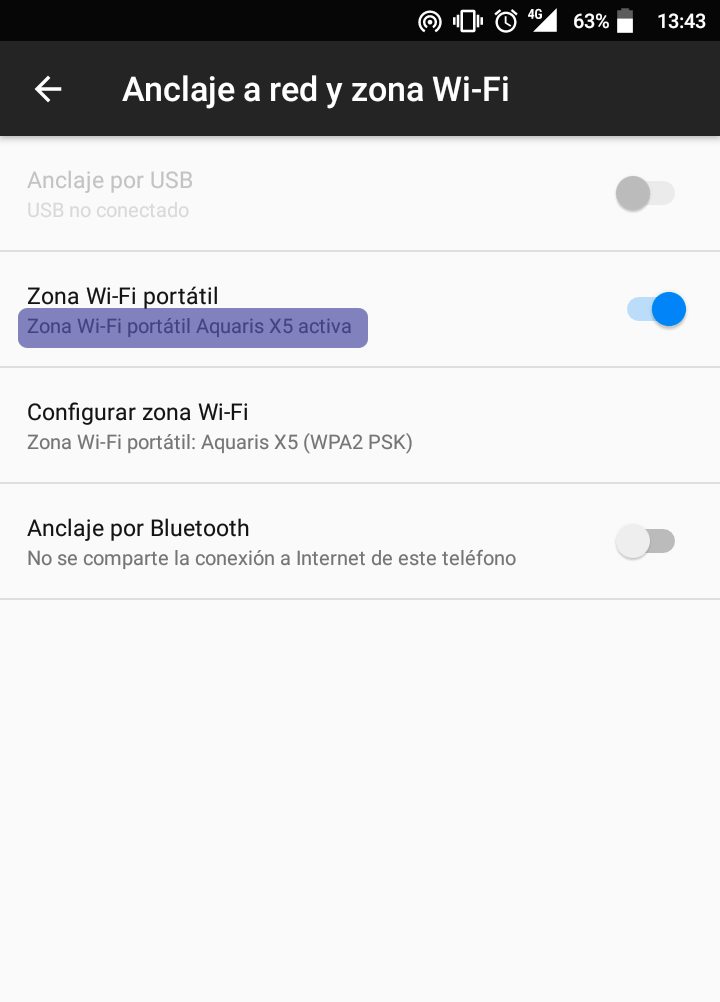
\includegraphics[scale=0.18]{6v2.png}
		\end{center}
		
	\end{block}
	
\end{columns}
\end{frame}

\begin{frame}{Ejemplo con Ettercap en red segura}
\begin{block}{Escenario}
	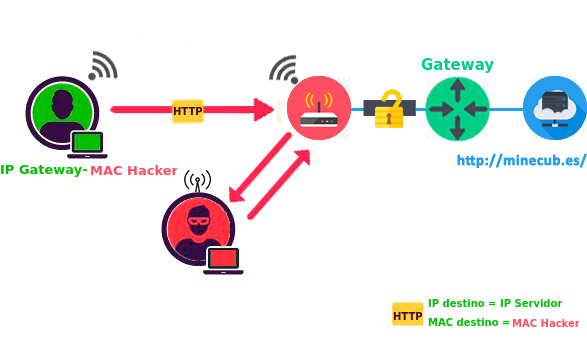
\includegraphics[scale=0.55]{Escenario.png}
\end{block}
\end{frame}

%\begin{frame}{Ejemplo con Ettercap en red segura}
%\begin{block}{Escenario}
%	\begin{center}
%		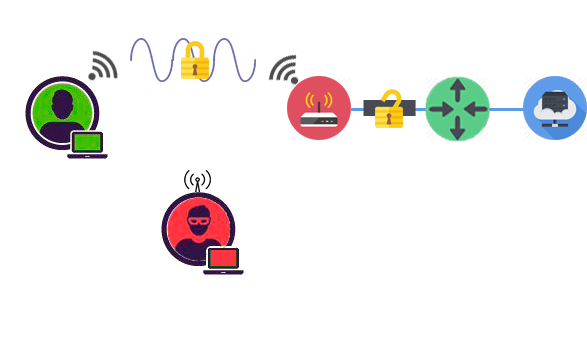
\includegraphics[scale=0.55]{wpayrouter.png}
%	\end{center}
%\end{block}
%\end{frame}


%\subsection{HTTPS}
\begin{frame}{¿Qué es HTTPS?}
\begin{block}{Definición}
	Es un protocolo de aplicación basado en el protocolo HTTP, destinado a la transferencia segura de datos de Hipertexto, es decir, es la versión segura de HTTP.
\end{block}
\begin{block}{¿Cómo funciona?}
	El sistema HTTPS utiliza un cifrado basado en SSL/TLS para crear un canal cifrado (cuyo nivel de cifrado depende del servidor remoto y del navegador utilizado por el cliente). De este modo se consigue que la información sensible no pueda ser usada por un atacante que haya conseguido interceptar la transferencia de datos de la conexión, ya que lo único que obtendrá será un flujo de datos cifrados que le resultará imposible de descifrar.
\end{block}
\end{frame}

%\subsection{SSLStrip}
%\begin{frame}{SSLStrip}
%\begin{block}{¿Qué es SSLStrip?}
%Es una aplicación capaz de descifrar el tráfico HTTPS que viaja a través de una red dejándolo visible en "texto plano".
%\end{block}
%\begin{center}
%
\includegraphics[scale=0.75]{https.png}
%\end{center}
%\end{frame}

%\subsection{HSTS}
%\begin{frame}{HSTS}
%\begin{block}{¿Qué es HSTS?}
%Es un protocolo de seguridad que deniega las conexiones HTTP y solo posibilita las comunicaciones HTTPS entre el cliente y el servidor.
%\end{block}
%\begin{block}{¿Cómo funciona?}
%Para poder activar esta utilidad, el usuario debe ser capaz de haber establecido una conexión al menos una vez de forma exitosa con dicha web.
%\end{block}
%\end{frame}

\subsection{No conocemos la passphrase}
\begin{frame}{Espionaje en red WPA2-PSK}
Se nos presentan dos situaciones:
\begin{enumerate}
	\item Conocemos la passphrase.
	\item \textbf{{\large No conocemos la passphrase.}}
\end{enumerate}
\end{frame}

\begin{frame}{Espionaje en red WPA2-PSK sin conocer la passphrase}
\begin{block}{KRACK}
	Key Reinstallation Attack: Se basa en forzar el reuso del SNonce de tal forma que se puedan desencriptar los datos. No es necesario el conocimiento de la clave Wi-Fi.
\end{block}

\end{frame}

\begin{frame}{Espionaje en red WPA2-PSK sin conocer la passphrase}
\begin{block}{Saludo de 4 vías de WPA2-PSK}
	\begin{center}
		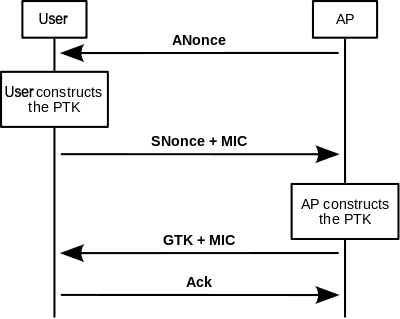
\includegraphics[scale=0.6]{Saludo4vias.png}
	\end{center}
\end{block}
\end{frame}


\begin{frame}{Espionaje en red WPA2-PSK sin conocer la passphrase}
\begin{block}{Recursos a usar en KRACK}
	\begin{itemize}
		\item Rogue-AP.
		\item Man-in-the-middle.
		\item Script KRACK.
		\item SSLStrip.
		\item Un sniffer.
		
	\end{itemize}
\end{block}
\begin{block}{Paso a paso}
\begin{enumerate}
	\item Montamos un Rogue-AP.
	\item Preparamos el Man-in-the-middle.
	\item Ordenamos un cambio de canal.
	\item Activamos el script KRACK.
	\item Abrimos el sniffer.
\end{enumerate}
\end{block}
\end{frame}

\begin{frame}{Gracias}
	\begin{center}
		
\includegraphics[scale=0.7]{Gracias.png}
	\end{center}
\end{frame}


\end{document}

